%Standardní zobrazovací řetězec a realizace jeho jednotlivých kroků. Gouraudovo a Phongovo stínování. Řešení viditelnosti. Grafický standard OpenGL: stručná charakteristika.
\subsection{Standardní zobrazovací řetěz}
Klade \textbf{důraz na rychlost }nikoli na kvalitu, realizuje ho \textbf{OpenGL}.
\begin{figure}[H]
\centering
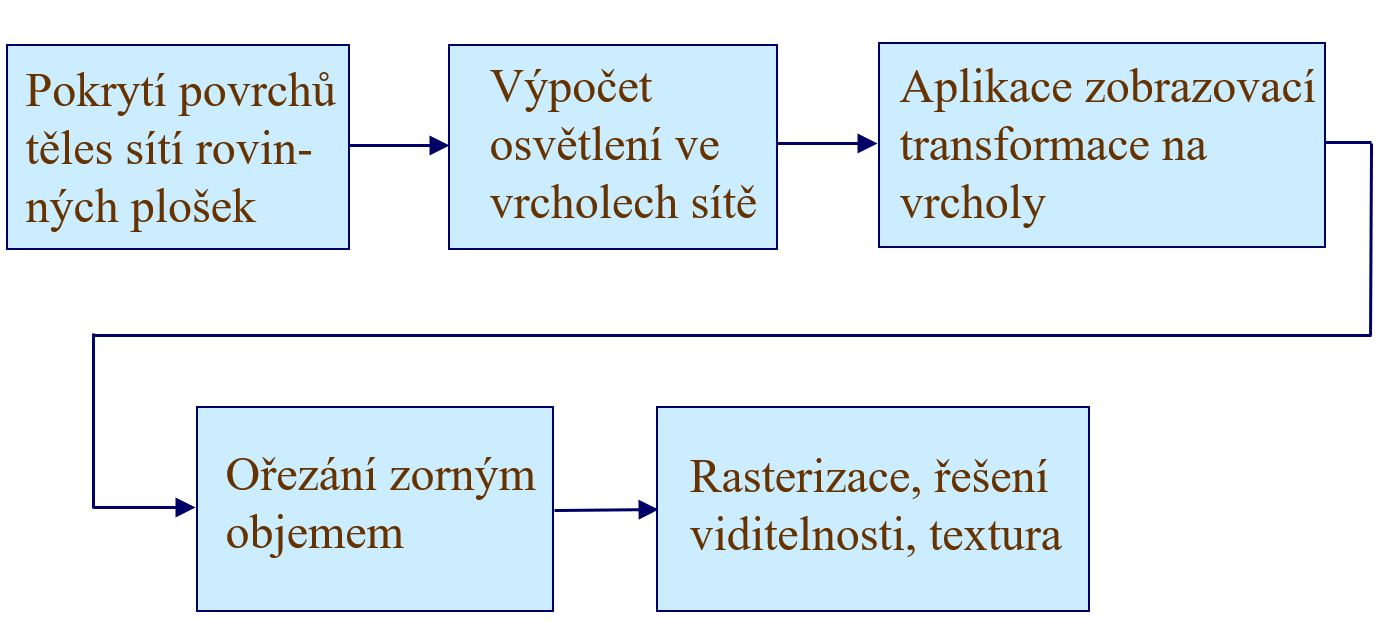
\includegraphics[width=0.75\textwidth]{assets/5_retezec}
\end{figure}

\begin{enumerate}
	\item  \textbf{Pokrytí povrchu objektů sítí rovinných plošek:}
	\begin{itemize}
		\item Ploškami bývají nejčastěji \textbf{trojúhelníky} nebo čtyřúhelníky.
		\item Pro objekty ve tvaru mnohostěnu je takové dělní vcelku samozřejmé.
		\item K \textbf{přesnějšímu výpočtu }barev bývá, ale někdy dělení na plošky \textbf{jemnější}.
		\item Někdy síť rovinných plošek žádaný povrch pouze aproximuje.
	\end{itemize}
	\item \textbf{Výpočet osvětlení ve vrcholech sítě} -- k tomu známe:
	\begin{itemize}
		\item Polohu, intenzitu a barvu světelných zdrojů.
		\item Souřadnice vrcholů ($P$), normál ($n$) a konstanty popisující optické vlastnosti materiálu ($O_a, O_d, O_s$).
		\item V tomto kroku je počítán barevný vjem každého vrcholu.
		\begin{figure}[H]
		\centering
		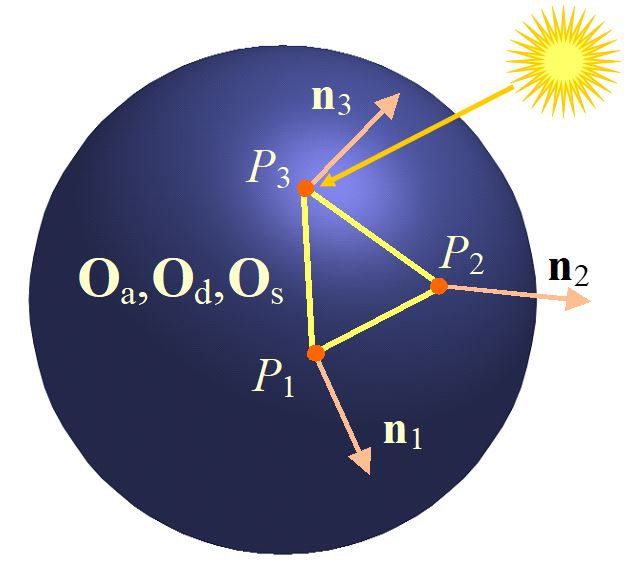
\includegraphics[width=0.4\textwidth]{assets/5_vypocet_barevneho_vjemu}
		\end{figure}
	\end{itemize}
	\item \textbf{Aplikace zobrazovací transformace na vrcholy}
	\begin{itemize}
		\item Oblíbenou technikou je středové promítání, to je zadáno:
		\begin{itemize}
			\item Polohou průmětny.
			\item Polohou středu promítání.
		\end{itemize}
		\begin{figure}[H]
		\centering
		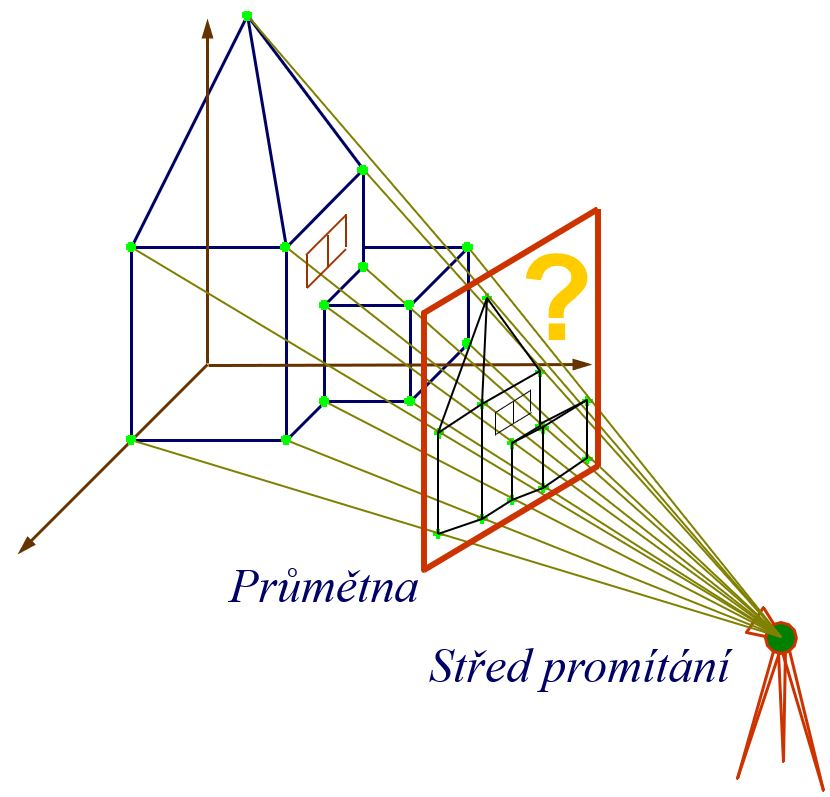
\includegraphics[width=0.5\textwidth]{assets/5_stred_promitani}
		\end{figure}
	\end{itemize}
	\item \textbf{Ořezání zorným objemem}
	\begin{itemize}
		\item Objekty nebo jejich části, nacházející se mimo zorný objem (obvykle jehlan) jsou odstraněny.
	\end{itemize}
		\begin{figure}[H]
		\centering
		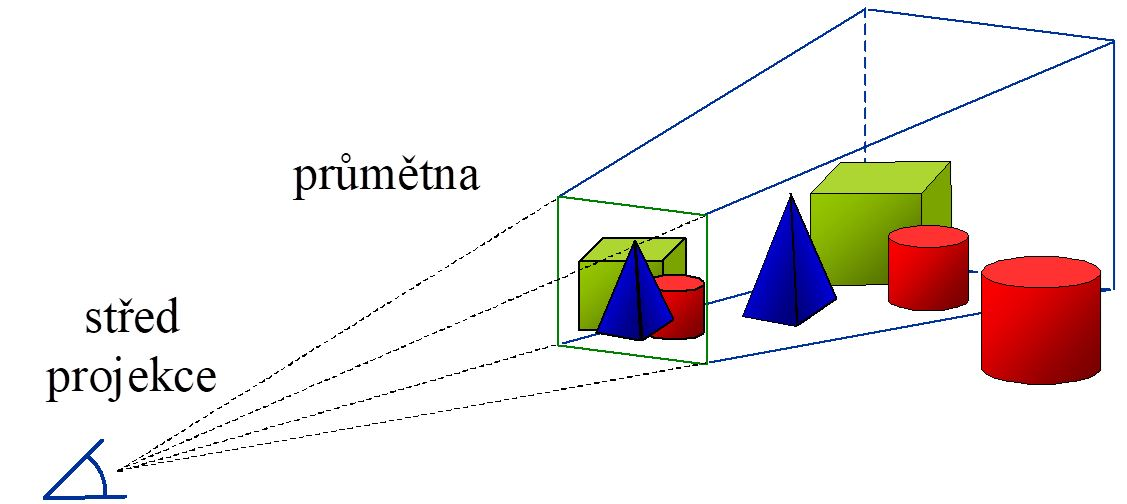
\includegraphics[width=0.5\textwidth]{assets/5_orezani_zornym_pole}
		\end{figure}
	%\begin{enumerate}
	\item \textbf{Rasterizace plošek}
	\begin{itemize}
		\item Postupně se zpracovávají všechny plošky.
		\item Pro každou plošku jsou ,,rozsvěceny'' všechny její pixely.
		\item Barva každého pixelu se stanoví \textbf{interpolací mezi hodnotami ve vrcholech}.
		\begin{figure}[H]
		\centering
		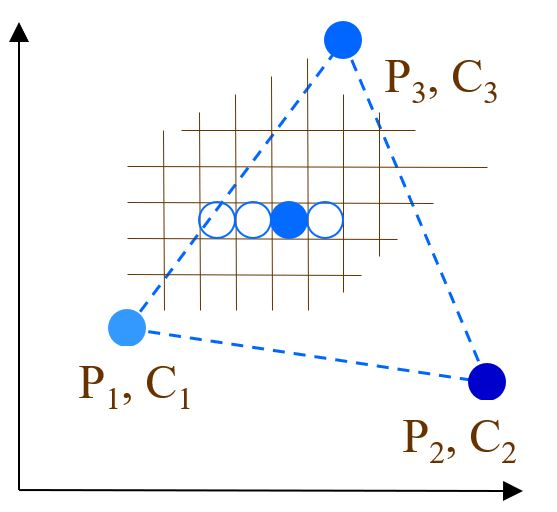
\includegraphics[width=0.5\textwidth]{assets/5_rasterizace_plosek}
		\end{figure}
	\end{itemize}
	\item[5.1] \textbf{Řešení viditelnosti (z--buffer)}
	\begin{itemize}
		\item Pro rozhodnutí viditelnosti se použijí hodnoty souřadnice $z$ (zde je $z_1 > z_2$).
		\item Před řešením viditelnosti bývá středové promítání převedeno na rovnoběžné.
		\begin{figure}[H]
		\centering
		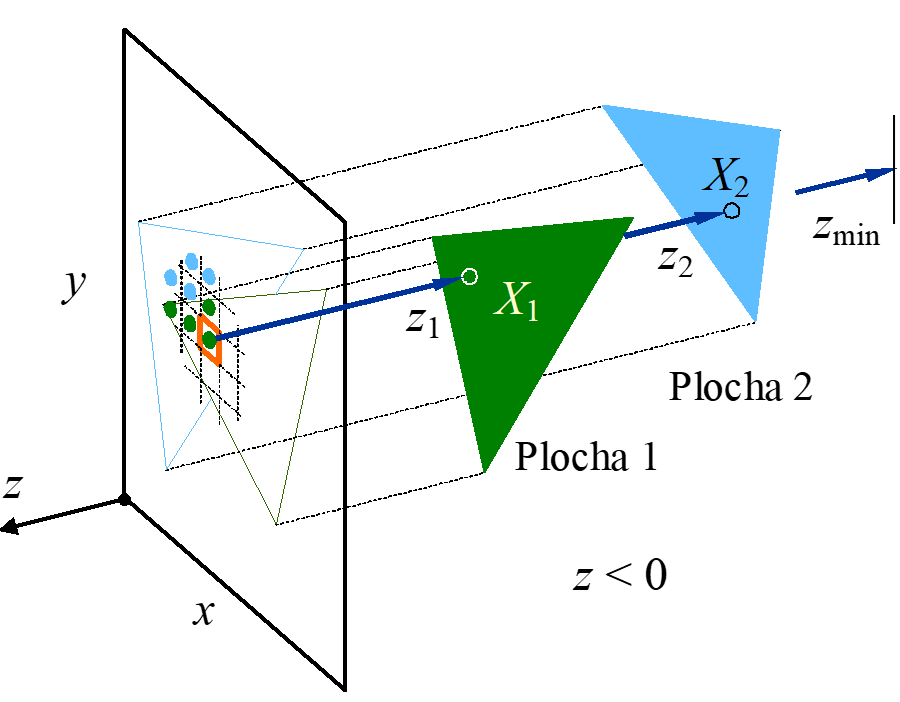
\includegraphics[width=0.5\textwidth]{assets/5_pip_zbuffer}
		\end{figure}
	\end{itemize}
	\item[5.2] \textbf{Nanášení textury}
	\begin{itemize}
		\item Vzhled obrázků lze vylepšit nánášením textury.
	\end{itemize}
\end{enumerate}

\subsection{Stínování (shading)}
\begin{itemize}
	\item Vykreslování barevných objektů \textbf{různými odstíny barev}.
	\item Lze odlišit křivosti ploch a tím docílit lepšího prostorového vjemu.
	\item Neplést s výpočtem vrženého stínu.
	\item Základní typy: \textbf{Konstantní} stínování, \textbf{Gouraudovo} stínování (Interpolace barvou), \textbf{Phongovo} stínování (Interpolace normálových vektorů).
\end{itemize}
\subsection{Gouraudovo stínování (Interpolace barvou)}
Princip metody spočívá v tom, že pokud budeme znát \textbf{normálu} v každém \textbf{vrcholu} každé plochy objektu, pak lze vypočítat barvu v tomto vrcholu a \textbf{interpolací} vypočítat \textbf{barvu pixelu uvnitř plošky} (bilineární interpolace).

Přesto ani tento způsob stínování neposkytuje zcela věrný obraz reálných objektů - interpolace samotného odstínu barvy totiž \textbf{nemůže} způsobit místní zvýšení jasu na plošce, stejně jako nemůže kvalitně vytvořit \textbf{odlesky} způsobené odraženým světlem. Dá se říci, že tato metoda zahlazuje barevné rozdíly u místních nerovností povrchu.

	\textbf{Normálový vektor} pro každý vrchol vypočteme jako aritmetický průměr normálových vektorů plošek, které se v tomto vrcholu stýkají.
\begin{figure}[H]
\centering
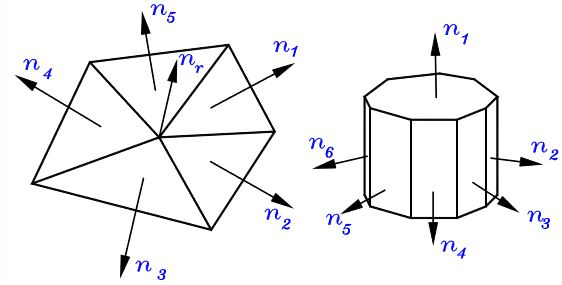
\includegraphics[width=0.5\textwidth]{assets/5_gouraud}
\end{figure}

\begin{enumerate}
	\item Vypočteme \textbf{normálové vektory pro všechny plošky} ze kterých je objekt složený.
	\item Pro každý vrchol spočítáme \textbf{normálový vektor} v tomto vrcholu jako \textbf{průměr normálových vektorů plošek}, které se v tomto vrcholu stýkají.
	\item Z normálových vektorů ve vrcholech a pozice světelného zdroje vypočteme \textbf{barvy ve vrcholech plošek}.
	\item Provedeme \textbf{interpolaci} barvy pro \textbf{body jednotlivých plošek}.
\end{enumerate}
		\begin{figure}[H]
		\centering
		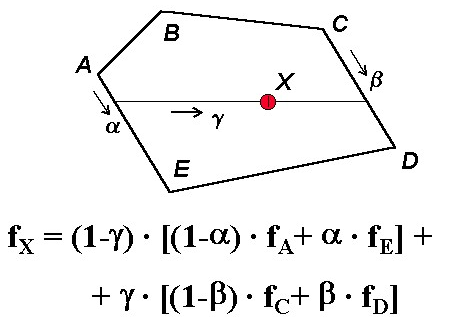
\includegraphics[width=0.4\textwidth]{assets/5_gouradovo}
		\end{figure} 
		\subsubsection*{Výhody}
			\begin{itemize}
				\item[$+$] umožnuje dobře zobrazit i hladké objekty,
				\item[$+$] používá se jako nejčastější metoda stínování.
			\end{itemize}
		\subsubsection*{Nevýhody}
			\begin{itemize}
				\item[$-$] nevznikají ostré odlesky uprostřed polygonů.
			\end{itemize}
\subsection{Phongovo stínování (Interpolace normálových vektorů)}
\begin{itemize}
	\item Provádí se \textbf{interpolace normálových vektorů} jednotlivých vrcholů, Interpolaci provádíme po řádcích.
	\item Touto metodou se \textbf{odstraní problém neostrých odlesků}.
	\item Je \textbf{náročnější} na výpočet než goraudovo stínování, jelikož se počítá výsledná barva v každém bodě plošky (ne pouze ve vrcholech).
	\item Pro normálové vektory lze psát:
		\begin{equation*} 
		\begin{split}
			n_A &= n_1 + (n_2 - n_1) \cdot u; \, u <0, 1>, \\
			n_B &= n_1 + (n_3 - n_1) \cdot w; \, w <0, 1>, \\
			n_Q &= n_A + (n_B - n_A) \cdot t; \, t <0, 1>, \\
		\end{split}
		\end{equation*}
\end{itemize}
		\begin{figure}[H]
		\centering
		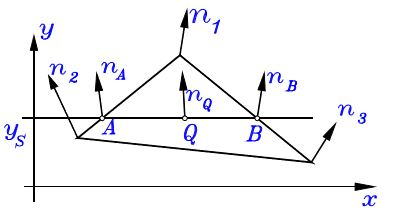
\includegraphics[width=0.5\textwidth]{assets/5_phong_stin}
		\end{figure}
\subsection{Řešení viditelnosti}
\begin{itemize}
	\item Podle výsledných dat:
	\begin{itemize}
		\item \textbf{Vektorové algoritmy} -- geometrické prvky vrcholy, hrany a stěny. Výstupem je vektorové řešení.
		\item \textbf{Rastrové algoritmy} -- výsledkem je rastrový obraz (jednotlivé pixely obsahují barvu), většina současných metod.
	\end{itemize}
	\item Podle místa řešení:
	\begin{itemize}
		\item \textbf{Řešení v prostoru objektů} -- proovnávání vzájemné polohy těles $0(n^2)$.
		\item \textbf{Řešení v prostoru obrazu} -- pracujeme s promítnutými a rasterizovanými objekty. Pro pixely hledáme nejbližší objekty.
	\end{itemize}
\end{itemize}

\subsubsection{Rastrové algoritmy}
\begin{enumerate}
	\item \textbf{Malířův algoritmus} (Painter's algorithm) -- porovnává plochy z hlediska jejich $z$--tových souřadnic (plocha s menší $z$--tovou souřadnící bude kreslena první), jestliže se plochy \textbf{nepřekrývají}, potom na pořadí kresby nezáleží, pokud se protínají -- rozdělit na nepřekrývající se plochy.
		\begin{figure}[H]
		\centering
		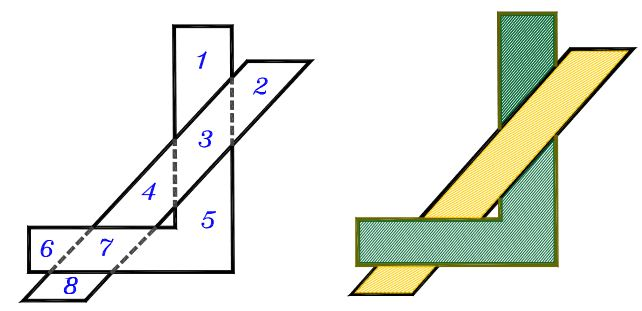
\includegraphics[width=0.5\textwidth]{assets/5_malir}
		\end{figure}
	\item \textbf{Dělení obrazovky }(Warnock subdivision)
		\begin{enumerate}
				\item Všechny plošky leží mimo zónu - zůstane barva pozadí.
				\item Oblast obsahuje právě jeden celý n-úhelník. Daná oblast se vyplní barvou a zbytek pozadím. 
				\item Oblast protíná právě jeden n-úhelník. Daná část se vyplní barvou, zbytek pozadí. 
				\item Pokud zobrazovaná část je celá uvnitř jednoho n-úhelníka, potom se celá oblast zobrazí barvou nejbližšího n-úhelníka, který oblast obklopuje. 
				\item Pokud nenastane jeden z vyjmenovaných případů - oblast se rozdělí.
		\end{enumerate}
		\begin{figure}[H]
		\centering
		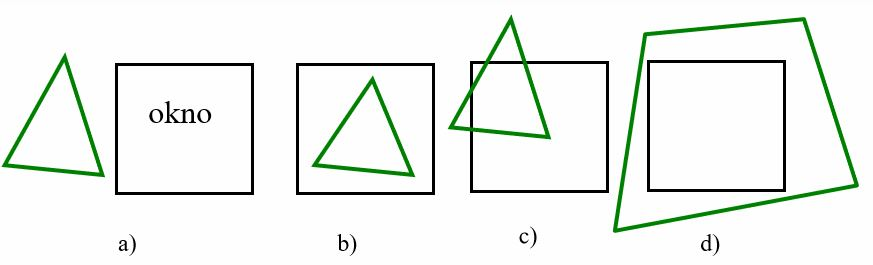
\includegraphics[width=0.5\textwidth]{assets/5_warnock}
		\end{figure}
	\item \textbf{Plovoucí horizont} (Floating Horizon Algorithm) -- metoda \uv{zig--zag}, počítáme od \uv{nejbližšího} rohu plochy k \uv{oku} pozorovatele.
		\begin{figure}[H]
		\centering
		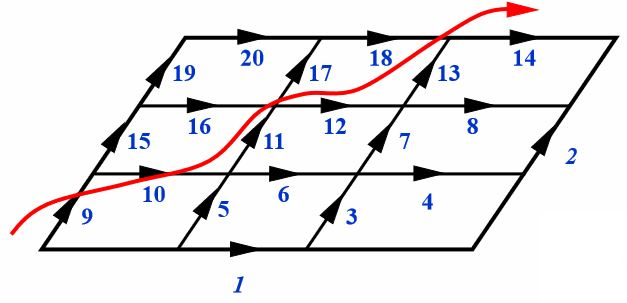
\includegraphics[width=0.5\textwidth]{assets/5_horizont}
		\end{figure}
	\item \textbf{Paměť hloubky} (\textbf{Z--buffer}, depth--buffer)
	\begin{enumerate}
				\item Vyplň obrazovou paměť barvou pozadí.
				\item Vyplň paměť hloubky -- nekonečnem.
				\item Pro každou plochu najdi její průměť (rasterizaci) nalezenému pixelu $[x_i,y_i]$ přiřaď hloubku $z_i$.
				\item Porovnej hloubku a zapiš do paměti, pokud je hloubka menší překreslí se nový pixel daným objektem.
	\end{enumerate}
		\begin{figure}[H]
		\centering
		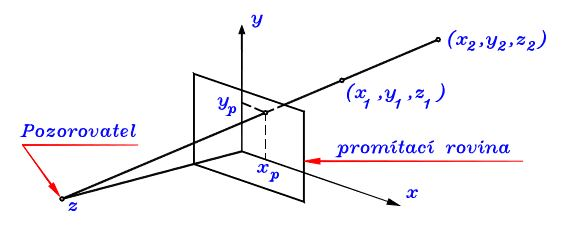
\includegraphics[width=0.7\textwidth]{assets/5_zbuffer}
		\end{figure}
		\begin{itemize}
		\item \textbf{Nejznámější} a \textbf{nejefektivnější} metoda.
		\item Každá plocha se zpracovává \textbf{pouze jednou}.
		\item \textbf{Doba zpracování roste s počtem ploch lineárně} (záleží i na velikosti ploch).
		\item Není potřeba žádné třídění nebo pomocné datové struktury.
		\item Možnost \textbf{paralelních} procesů.
		\item Z-buffer je často realizován jako 2D pole, kdy se ukládá pouze aktuální hodnota z (nejmenší).
		\end{itemize}
	\item \textbf{Z--buffer -- paměť hlouby -- průhlednost - princip}
	\begin{enumerate}
		\item Inicializuj \textbf{color buffer} a \textbf{depth buffer}.
		\item Postupně načti všechny plochy, neprůhledné zpracuj, průhledné si zapamatuj a odlož pro následné zpracování.
		\item Po zpracování neprůhledných ploch setřiď průhledné plochy podle vzdálenosti.
		\item Zpracuj průhledné plochy s použitím \textbf{alfa míchání}.
	\end{enumerate}
\end{enumerate}
\subsection{Grafický standard OpenGL: stručná charakteristika}
\begin{itemize}
\item OpenGL je \textbf{multiplatformní} standard poskytující rozhraní (\textbf{API}) pro zobrazování 2D a 3D objektů. Je podporován takřka všemi výrobci grafických karet.
\item Používá se pro tvorbu \textbf{PC Her}, \textbf{CAD programů}, aplikací \textbf{virtuální reality} či pro  \textbf{vědecko-techické vizualizace}.
\item Veškerá činnost OpenGL se řídí vykonáváním příkazů pomocí \textbf{volání funkcí} a procedur (kterých je v OpenGL cca 250).
\item Byla vytvořena tak, aby byla \textbf{nezávislá} na použitém \textbf{operačním systému} nebo \textbf{programovacím jazyce}. Specifikace OpenGL tedy \textbf{neříká nic} o řízení kontextu platformy, \textbf{správě} a vytváření \textbf{oken}, \textbf{audio} a \textbf{vstupu}. Řešení této problematiky je necháno na \textbf{podpůrných systémech} (které jsou většinou platformě specifické) a OpenGL se zabývá pouze vykreslováním.
\item Z programátorského hlediska se OpenGL chová jako \textbf{stavový automat}. To znamená že pokud změníme nějaké nastavení, toto nastavení zůstane až do doby než jej znovu změníme. To se hodí např. kdy jediným příkazem jsme schopni přepnout program do kreslení ve ,,wireframe módu''.
\item Programátorské rozhraní knihovny OpenGL je vytvořeno tak, aby knihovna byla použitelná v téměř \textbf{libovolném programovacím jazyce}. Primárně je k dispozici hlavičkový soubor pro jazyky C a C++. Existují však i podobné soubory s deklaracemi pro další programovací jazyky, například Fortran, Object Pascal či Javu; tyto soubory jsou většinou automaticky vytvářeny z Cčkovských hlavičkových souborů.
\end{itemize}

\subsubsection{Core-profile vs Immediate mode}
Ve starších verzích OpenGL (před 3.2, kde se stal deprecated) se vyvíjely aplikace v tzv. \textbf{immediate módu} (non-shader mód). Tento mód byl značně \textbf{jednodušší} než core-profile, jelikož zakrýval (abstrahoval) většinu funkcionality OpenGL pod danou knihovnu, za to však zaplatil svou \textbf{neefektivitou}. To je způsobeno (mimo jiné) tím, že při každé specifikaci vertexu je jeho pozice odeslána na GPU, což představuje bottleneck v komunikaci mezi CPU a GPU. Tento mód lze stále použít v moderním OpenGL pokud využíváme tzv. \textbf{compatibility profile}.

Moderní OpenGL tedy nutí uživatele využívat moderní praktiky, přičemž pokud se snaží využívat starých metod, OpenGL vyhodí chybu a přestane vykreslovat. Přestože je core-profile na první pohled značně \textbf{složitější}, je \textbf{efektivnější}, umožňuje \textbf{větší flexibilitu} a \textbf{lepší porozumění grafického programování}. Core-profile přináší \textbf{buffer objecty} a je založen převážně na použití \textbf{shaderů}, které jsou vždy zkompilované do malých podprogramů na CPU a \textbf{nahrány na GPU pouze jednou}.

\begin{figure}[H]
	\centering
	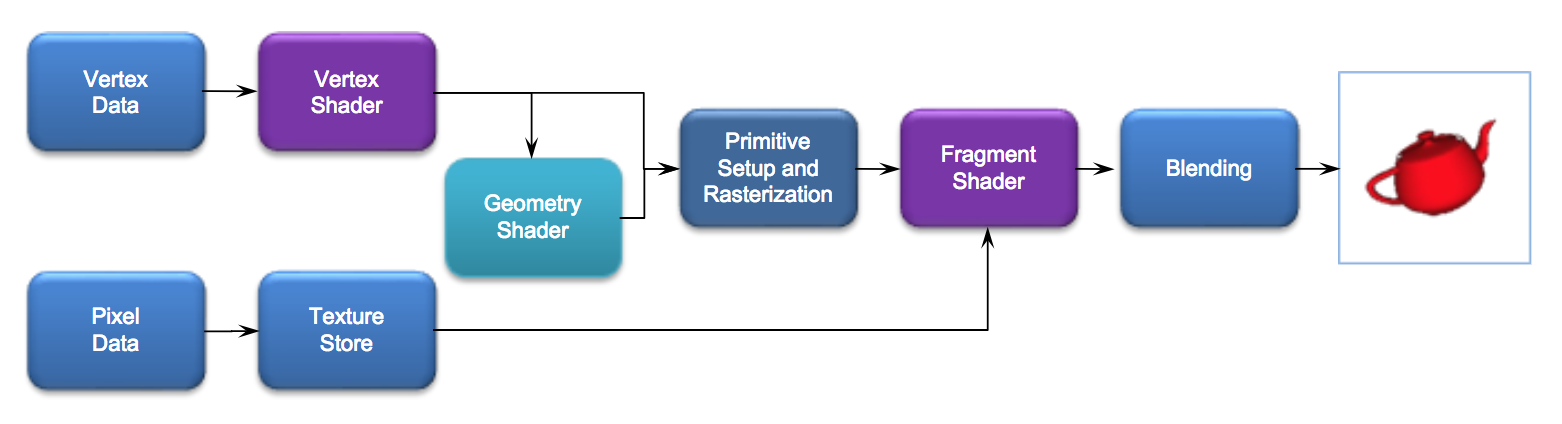
\includegraphics[width=\textwidth]{assets/5_opengl_pipe}
\end{figure}

Od verze 4.1 přibyla ještě mezi vertex a geometry shader fáze \textbf{Tessalace}.

\begin{minted}{glsl}
// ..:: Initialization code :: ..
// 1. bind Vertex Array Object
glBindVertexArray(VAO);
// 2. copy our vertices array in a vertex buffer for OpenGL to use
glBindBuffer(GL_ARRAY_BUFFER, VBO);
glBufferData(GL_ARRAY_BUFFER, sizeof(vertices), vertices, GL_STATIC_DRAW);
// 3. copy our index array in a element buffer for OpenGL to use
glBindBuffer(GL_ELEMENT_ARRAY_BUFFER, EBO);
glBufferData(GL_ELEMENT_ARRAY_BUFFER, sizeof(indices), indices, GL_STATIC_DRAW);
// 4. then set the vertex attributes pointers
glVertexAttribPointer(0, 3, GL_FLOAT, GL_FALSE, 3 * sizeof(float), (void*)0);
glEnableVertexAttribArray(0);  

[...]

// ..:: Drawing code (in render loop) :: ..
glUseProgram(shaderProgram);
glBindVertexArray(VAO);
glDrawElements(GL_TRIANGLES, 6, GL_UNSIGNED_INT, 0)
glBindVertexArray(0);
\end{minted}

\subsubsection{GLSL (OpenGL Shading Language)}
Je součástí OpenGL 2.0 a vyšší. Jedná se o jazyk pro programování shaderů, který je syntaxí velice podobný C. Shadery jsou malé programy, které běží na GPU. Jeho vlastnosti:
\begin{itemize}
\item Definuje \textbf{speciální proměnné} \texttt{gl\_Position} (výstupní pozice z vertex shader) a \texttt{gl\_FragColor} (výstupní barva z fragment shaderu).
\item \textbf{Datové typy}: vektory, matice, int, float, bool, C-like structures.
\item Předávání hodnot mezi vertex/geometry/fragment shadery lze pomocí \textbf{vstupních} a \textbf{výstupních} \textbf{proměnných} \texttt{in, out, inout}.
\item Možnost vytváření vlastních \textbf{funkcí} (default funkce musí být \texttt{main()}).
\end{itemize}




